% Equipo 42 - Route Intelligence. Versión definitiva para entrega, 15 noviembre 2026.
% Basado en la plantilla institucional del Producto de difusión.
% Compilación Overleaf: pdfLaTeX + Biber + pdfLaTeX (dos pasadas).
\documentclass[letterpaper,11pt]{article}
\usepackage[utf8]{inputenc}
\usepackage[T1]{fontenc}
\usepackage{lmodern}
\usepackage[spanish,es-tabla]{babel}
\decimalpoint
\usepackage[margin=2.5cm]{geometry}
\usepackage{setspace}\setstretch{1.14}
\usepackage{microtype}
\usepackage{graphicx,booktabs,float,array,amsmath,amssymb}
\usepackage[font=small,labelfont=bf,labelsep=colon]{caption}
\usepackage{fancyhdr,titlesec}
\geometry{headheight=52pt,headsep=0.3cm}
\renewcommand{\headrulewidth}{0pt}
\fancypagestyle{plain}{\fancyhf{}\fancyhead[C]{
\includegraphics[height=1.2cm]{logo.jpeg}}\fancyfoot[C]{\thepage}}
\pagestyle{fancy}\fancyhf{}\fancyfoot[C]{\thepage}
\titleformat{\section}{\Large\bfseries}{\thesection.}{0.6em}{}
\titleformat{\subsection}{\large\bfseries}{\thesubsection.}{0.6em}{}
\titlespacing*{\section}{0pt}{1.6ex plus .4ex}{.8ex}
\titlespacing*{\subsection}{0pt}{1.2ex plus .3ex}{.5ex}
\usepackage{csquotes}
\usepackage[style=apa,backend=biber]{biblatex}
\addbibresource{referencias.bib}
\addbibresource{referencias_adicionales.bib}
\usepackage[hidelinks]{hyperref}\urlstyle{same}
\newcommand{\K}{K=32}
\newcommand{\Muno}{M1}
\newcommand{\MAE}{\mathrm{MAE}}
\newcommand{\WAPE}{\mathrm{WAPE}}
\newcommand{\citaexp}[1]{\textit{#1}}
\title{\textbf{Estimación y pronóstico de tiempos de viaje en redes dirigidas}\\[4pt]
\large Matrices experimentales para la planeación y recuperación de rutas\\[3pt]
\normalsize Estudio con datos derivados de PEMS-BAY}
\author{Luis Ángel Herrera Flores \quad Francisco Natanael Ortiz Martínez\\ Edgar Iván Rosas Gómez\\[6pt]
\normalsize Proyecto Integrador · Maestría en Inteligencia Artificial Aplicada\\[3pt]
\normalsize Tecnológico de Monterrey · Equipo 42 -- Route Intelligence\\[3pt]
\normalsize Asesor: Dr. Gerardo Jesús Camacho González · 15 de noviembre de 2026}
\date{\vspace{-2ex}}
\begin{document}
\maketitle
\begin{abstract}

En la planeación y recuperación de rutas con ventanas de tiempo, es habitual utilizar estimaciones de los tiempos de viaje entre ubicaciones, los cuales pueden variar según las condiciones de circulación. Se desarrollaron y evaluaron dos procedimientos para generar matrices de tiempos origen--destino (OD) sobre una red experimental dirigida derivada de PEMS-BAY, integrada por 322 nodos y 345 aristas. El modelo lineal residual M1 pronostica los tiempos de viaje de la jornada siguiente, entre las 08:00 y las 15:55, con información disponible hasta las 18:00 del día anterior. En junio de 2017, sobre 13 macronodos (puntos funcionales de conexión vial), redujo el error absoluto medio (MAE) OD de 38.15 a 32.67 segundos (14.36\,\%) respecto de una referencia histórica. La reconstrucción contemporánea mediante Ridge con $K=32$ combina información histórica y 32 consultas OD simuladas del instante objetivo. En junio de 2017, redujo el MAE OD de 31.75 a 11.42 segundos (64.04\,\%) respecto de la referencia histórica, en cinco grupos de 20 sensores. Ambos procedimientos se evaluaron bajo condiciones de información y protocolos diferentes, por lo que sus resultados no son directamente comparables. En este entorno experimental, las consultas OD se simularon sin ruido de medición y se obtuvieron matrices de tiempos de viaje exportables. La evaluación también permitió identificar mayores errores bajo condiciones de circulación lenta, lo que señala una oportunidad de mejora para los procedimientos desarrollados. La integración de estas matrices en un modelo de optimización y la evaluación de sus efectos sobre las rutas se plantean como líneas de trabajo futuro.
\end{abstract}
\noindent\textbf{Palabras clave:} tiempos de viaje, reconstrucción de matrices OD, pronóstico anticipado, redes dirigidas, PEMS-BAY.

\section{Introducción y planteamiento del problema}
\subsection{Ruteo con ventanas de tiempo y variación de la movilidad}

En la planeación de rutas de distribución se consideran, entre otros elementos, las ubicaciones que deben visitarse, la capacidad de los vehículos y los horarios de atención. Cuando se establecen intervalos dentro de los cuales debe atenderse a cada cliente, se plantea una variante conocida como problema de ruteo de vehículos con ventanas de tiempo (VRPTW, por sus siglas en inglés) \parencite{solomon1987}. Una de las entradas habituales de estos modelos es una matriz que contiene los tiempos estimados de desplazamiento entre pares de ubicaciones. Sin embargo, la duración de los viajes puede variar según las condiciones de circulación y el horario de salida, como se reconoce en los modelos de ruteo dependientes del tiempo \parencite{malandraki1992,ichoua2003}. Cuando los tiempos efectivos difieren de los estimados, pueden producirse cambios en los horarios de llegada y en el cumplimiento de las ventanas de servicio. Las consecuencias dependen de las características de cada ruta y de los márgenes de tiempo disponibles.

Un antecedente central del proyecto es la tesis de \textcite{berth2025} y el artículo de \textcite{berthtrigos2025}, que estudian la recuperación de rutas con ventanas de tiempo ante interrupciones durante su ejecución. Estos trabajos desarrollan un enfoque de optimización que permite revisar una planeación cuando cambian las condiciones consideradas inicialmente, tomando en cuenta el estado de avance de la operación y los servicios pendientes. También examinan las implicaciones de distintas políticas de recuperación para los actores involucrados. En este contexto, los tiempos de desplazamiento constituyen información relevante tanto para establecer la planeación inicial como para evaluar posibles ajustes durante su ejecución.

La variabilidad de los tiempos de viaje ha motivado el desarrollo de métodos para estimar y pronosticar las condiciones de circulación. Entre los enfoques estudiados se encuentran modelos que aprovechan patrones temporales y relaciones espaciales entre distintos puntos de una red vial \parencite{li2018,wu2019}. Esta línea de investigación resulta pertinente para el ruteo, ya que las condiciones del tráfico influyen en los tiempos de desplazamiento utilizados para planear los recorridos.

Las estimaciones de tiempos de viaje pueden utilizarse en distintos momentos de decisión. Antes del inicio de una jornada interesa anticipar las condiciones de circulación, mientras que durante su ejecución puede ser necesario actualizar las estimaciones a partir de información reciente. Para atender estas dos necesidades, se desarrollan y evalúan procedimientos diferentes sobre una red vial experimental. El pronóstico anticipado M1 utiliza información histórica para estimar los tiempos de la jornada siguiente; la reconstrucción contemporánea mediante Ridge con $K=32$ combina información histórica con consultas origen--destino (OD) simuladas del instante que se busca reconstruir. Ambos procedimientos generan matrices de tiempos de viaje que podrían utilizarse como insumos para la planeación o recuperación de rutas. La evaluación se concentra en la precisión de estas estimaciones y no comprende sus efectos sobre las soluciones obtenidas mediante optimización.

\subsection{Alcance y criterios de evaluación}\label{sec:alcance}

El objeto común de los dos procedimientos son los tiempos de desplazamiento entre ubicaciones de una red vial experimental. Los orígenes y destinos corresponden a puntos seleccionados de esa red, que no representan necesariamente establecimientos o clientes de una operación de distribución. Por tanto, se estudian tiempos calculados sobre la red y no duraciones observadas de viajes realizados por vehículos de reparto.

Aunque ambos procedimientos buscan estimar estos tiempos, se distinguen por el momento al que corresponden las estimaciones y por la información disponible. En el pronóstico para la jornada siguiente (M1), se estiman los tiempos de desplazamiento correspondientes al periodo de 08:00 a 15:55, utilizando únicamente información disponible hasta las 18:00 del día anterior, cuya última observación admisible corresponde a las 17:55. En la reconstrucción contemporánea ($K=32$), el parámetro $K$ representa el número de consultas origen--destino (OD) disponibles. Cada consulta proporciona el tiempo de desplazamiento entre dos puntos seleccionados de la red en el instante que se busca reconstruir. Para este componente se utilizan 32 consultas simuladas a partir del entorno experimental, junto con información histórica. Así, aunque ambos procedimientos generan matrices de tiempos de viaje, sus horizontes de estimación y conjuntos de información son diferentes.

La evaluación de ambos procedimientos se concentra en los errores de estimación respecto de los tiempos de referencia construidos para la red experimental. En M1 se analiza inicialmente el error por arista y posteriormente el de las matrices OD; en $K=32$, la evaluación principal se concentra en los tiempos OD de los pares evaluados. Se consideran el error absoluto medio (MAE), el error porcentual absoluto ponderado (WAPE), el percentil 95 del error absoluto (P95), el sesgo y la frecuencia de subestimación. Debido a las diferencias entre sus conjuntos de información y protocolos de evaluación, los errores de M1 y $K=32$ no deben interpretarse como una comparación directa de desempeño. Tampoco se establecieron umbrales previos de aceptación para una operación real ni se evaluó el efecto de las matrices sobre la factibilidad o la calidad de las rutas calculadas por un optimizador.

\section{Datos y construcción del entorno experimental}

\subsection{Fuente, cobertura y construcción de tiempos de viaje}

\paragraph{Fuente y depuración.}
Se utilizaron registros históricos de velocidad del conjunto de datos PEMS-BAY, derivado del sistema Performance Measurement System (PeMS) del California Department of Transportation \parencite{caltrans,li2018}. Los datos corresponden al periodo de enero a junio de 2017 y contienen 52\,116 instantes de observación, con una frecuencia nominal de cinco minutos. Las velocidades están expresadas originalmente en millas por hora y proporcionan la información de tráfico utilizada para construir los tiempos de desplazamiento de la red experimental.

La inspección inicial no identificó valores ausentes en la matriz original. Sin embargo, se encontraron 521 registros con velocidad igual a cero, concentrados en cuatro instantes. Estos valores se consideraron anómalos y se trataron como datos faltantes, sustituyéndolos mediante interpolación temporal entre observaciones válidas del mismo sensor. El procedimiento de depuración se encuentra documentado en los materiales técnicos identificados en el Apéndice~\ref{app:traza}.

También se examinó la continuidad de los registros temporales. Se identificó la ausencia de 12 intervalos de cinco minutos, correspondientes al periodo de las 02:00 a las 02:55 del 12 de marzo de 2017. Esta discontinuidad coincide con el inicio del horario de verano en California, cuando el reloj se adelanta una hora, por lo que no corresponde a una pérdida de observaciones de tráfico.

\paragraph{Red experimental.}
El conjunto original comprende 325 sensores distribuidos en distintos tramos de autopistas del área de la Bahía de San Francisco. Para construir la red experimental, se organizaron en 16 corredores dirigidos, cada uno formado por sensores ordenados según su ubicación y sentido de circulación. A partir de esta organización se establecieron conexiones entre sensores consecutivos, que representan segmentos de desplazamiento dentro de un mismo corredor.

Para representar las conexiones entre corredores se incorporaron 13 \emph{macronodos}. Estos nodos adicionales representan funcionalmente zonas de intercambio entre vías, sin reproducir de manera individual cada rampa o maniobra de incorporación. Su ubicación y las conexiones propuestas se examinaron con apoyo de OpenStreetMap \parencite{osm}, aunque no se verificaron exhaustivamente todos los movimientos vehiculares permitidos.

Para los experimentos se conservó el componente fuertemente conexo principal de la red, es decir, el conjunto de nodos entre los cuales existen caminos dirigidos en ambos sentidos. Esta selección comprende 309 sensores y los 13 macronodos, para un total de 322 nodos; los otros 16 sensores quedaron fuera del grafo utilizado. La red resultante contiene 345 aristas dirigidas, de las cuales 273 representan segmentos de corredor y 72 corresponden a conexiones auxiliares asociadas con los macronodos.

\paragraph{Tiempos por arista.}
Para asignar tiempos de desplazamiento a las aristas fue necesario estimar sus longitudes y las velocidades de circulación correspondientes. En los segmentos de corredor, las longitudes se obtuvieron a partir de diferencias entre marcadores de distancia vial (\emph{postmile}), convertidas de millas a kilómetros. Cuando un macronodo se incorporó entre dos sensores consecutivos, la longitud del segmento original se repartió entre las dos nuevas conexiones, considerando la ubicación geográfica del macronodo respecto de ambos sensores. En cambio, cuando la conexión se encontraba en un extremo del corredor, sin un segmento original que pudiera dividirse, su longitud se aproximó mediante la distancia geodésica entre el macronodo y el sensor correspondiente.

Las velocidades asignadas también dependen del tipo de arista. Cuando una conexión une dos sensores, se utiliza el promedio de las velocidades registradas en sus extremos. Para las conexiones que involucran un macronodo, se emplea la velocidad del sensor asociado. Con las longitudes estimadas y las velocidades convertidas a kilómetros por hora, se calculan los tiempos de desplazamiento por arista, expresados en minutos.

Estos tiempos constituyen estimaciones derivadas de los registros de velocidad y de las aproximaciones geométricas adoptadas para construir la red. No representan mediciones independientes de viajes completos entre orígenes y destinos. El procedimiento utilizado para calcular estos últimos a partir de los tiempos por arista se describe en la siguiente subsección.

\begin{figure}[!htb]
\centering
\begin{minipage}[t]{0.48\linewidth}
\centering
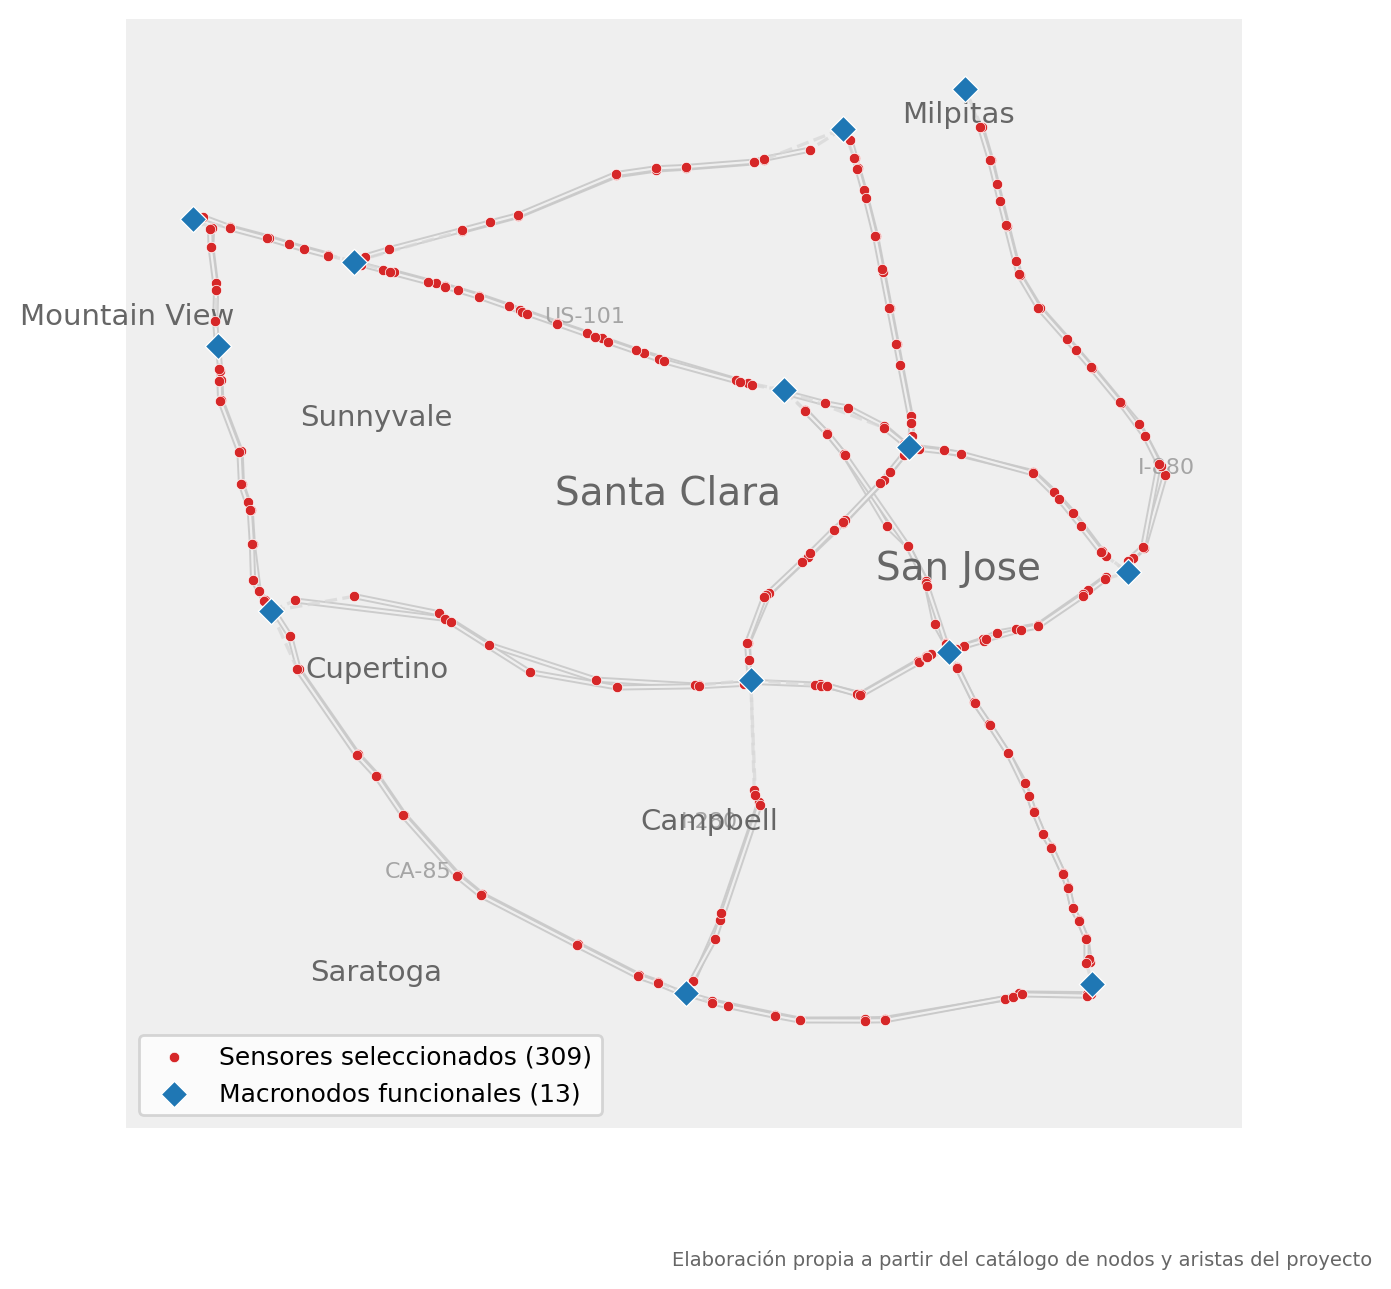
\includegraphics[width=\linewidth]{mapa_sensores_experimentales.png}
\end{minipage}\hfill
\begin{minipage}[t]{0.48\linewidth}
\centering
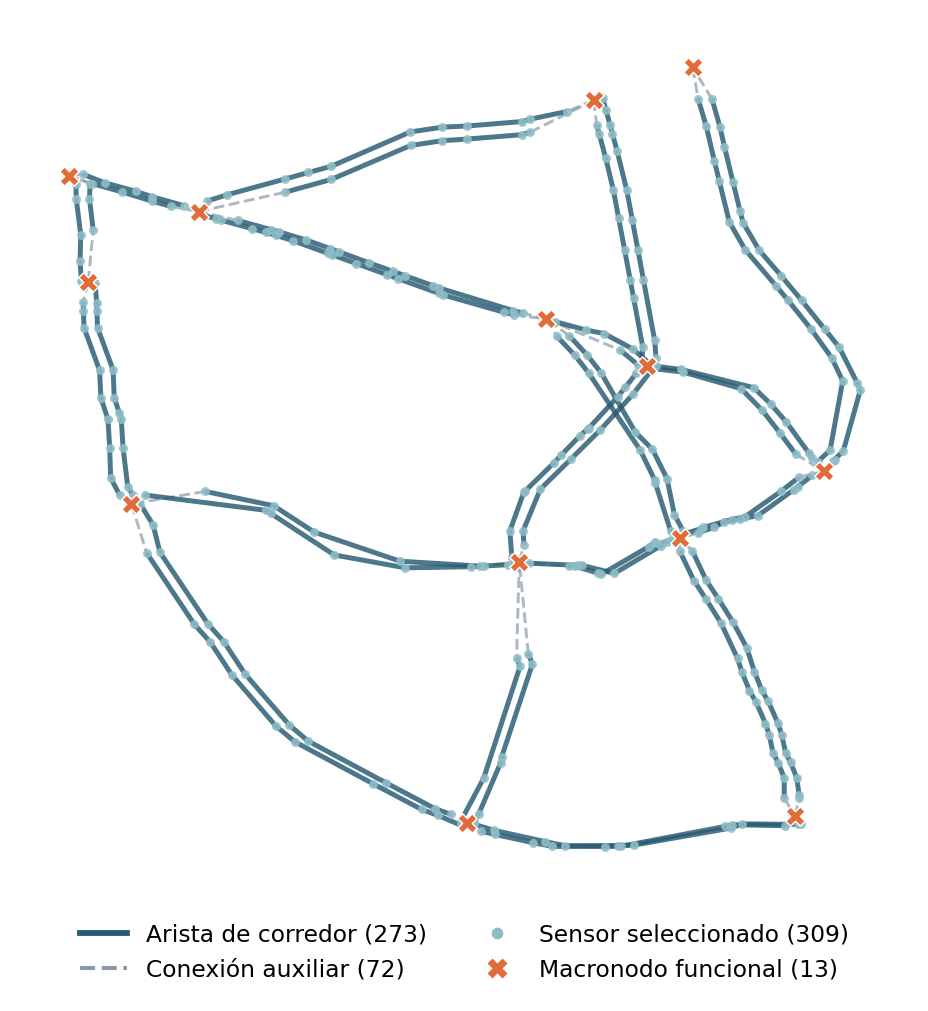
\includegraphics[width=\linewidth]{red_experimental_322_nodos.png}
\end{minipage}
\caption{Dos vistas complementarias de la red experimental. Izquierda: localización geográfica esquemática de los 309 sensores seleccionados y los 13 macronodos funcionales, elaborada a partir de las coordenadas del catálogo del proyecto; los nombres urbanos se incluyen solo como referencia espacial. Derecha: representación del grafo dirigido utilizado en los experimentos, con 345 aristas (273 de corredor y 72 auxiliares). Las posiciones son aproximadas y se separan ligeramente los sentidos de circulación con fines gráficos; ninguna de las dos vistas constituye una validación cartográfica exhaustiva de todos los movimientos vehiculares reales.}\label{fig:red}
\end{figure}

\subsection{Red dirigida y construcción de matrices OD}

La red experimental se representa mediante un grafo dirigido $G=(V,E)$, donde $V$ es el conjunto de nodos y $E$ el de aristas. A cada arista $e$ se le asigna un tiempo de desplazamiento $\tau_e(t)>0$, que depende de las condiciones de circulación registradas en el instante $t$. A partir de estos tiempos se construyen matrices origen--destino (OD), cuyos elementos representan la duración estimada del desplazamiento entre dos nodos de la red. Este desplazamiento puede comprender varias aristas y no necesariamente corresponde a una conexión directa entre el origen y el destino.

Para calcular cada elemento de la matriz se identifica el camino dirigido con menor tiempo de desplazamiento entre los nodos $i$ y $j$. Formalmente, el tiempo de referencia se define como:

\begin{equation}
T_{ij}(t)=\min_{p\in\mathcal{P}_{ij}}\sum_{e\in p}\tau_e(t),
\label{eq:od}
\end{equation}

donde $\mathcal{P}_{ij}$ representa el conjunto de caminos dirigidos que conectan ambos nodos dentro de la topología experimental. El cálculo se realiza mediante el algoritmo de Dijkstra, aplicable a grafos con pesos no negativos \parencite{dijkstra1959}. Debido a que la red conserva los sentidos de circulación, los caminos disponibles y sus duraciones pueden diferir según la dirección del desplazamiento. Por tanto, el tiempo estimado de $i$ a $j$ no tiene por qué coincidir con el de $j$ a $i$.

Los tiempos OD se calculan mediante una aproximación \emph{snapshot}: para cada instante evaluado se utilizan los tiempos por arista correspondientes a ese momento, suponiendo que permanecen constantes durante todo el desplazamiento. De esta manera, cada matriz representa las condiciones de circulación de un instante determinado, sin considerar los cambios que podrían producirse mientras un vehículo recorre la red. Esta simplificación permite establecer una referencia para evaluar los procedimientos de estimación, aunque no reproduce la evolución temporal del tráfico durante cada viaje.

La Figura~\ref{fig:red} presenta dos vistas de la red experimental: la ubicación geográfica aproximada de sus nodos y su representación como grafo dirigido. Esta última permite observar las conexiones que determinan los caminos disponibles entre orígenes y destinos. A partir de esta red se calculan matrices OD para distintos conjuntos de ubicaciones, seleccionados de acuerdo con los objetivos de cada evaluación. Los criterios de selección y las características de estos conjuntos se describen en las secciones de metodología y resultados.

\subsection{Particiones temporales y controles de fuga}
Los procedimientos de reconstrucción contemporánea y pronóstico se desarrollaron con particiones temporales diferentes. Para la reconstrucción, los pares origen--destino utilizados como consultas guía se seleccionaron a partir de información de enero a marzo de 2017. Abril y mayo se emplearon para explorar configuraciones y comparar modelos. Posteriormente, el modelo Ridge seleccionado se ajustó con datos de enero a mayo y se evaluó en junio. Las comparaciones adicionales de ensambles utilizaron nuevamente información de mayo, por lo que sus resultados en ese mes deben interpretarse como evidencia exploratoria y no como una evaluación independiente.

En el pronóstico para la jornada siguiente, las referencias históricas y los modelos se ajustaron inicialmente con datos de enero a marzo. La validación comenzó el 2 de abril, de manera que los pronósticos evaluados se emitieran después de concluido el periodo de entrenamiento. Abril también se utilizó para seleccionar el número de épocas de entrenamiento de los modelos neuronales. Los resultados de mayo y junio se emplearon para analizar el comportamiento de los modelos bajo distintas condiciones de circulación. Dado que ambos meses fueron examinados durante el desarrollo, estas evaluaciones tienen un carácter diagnóstico y no constituyen pruebas completamente ciegas.

En este segundo componente, cada pronóstico se formula con la información disponible hasta las 18:00 del día anterior, siendo las 17:55 la hora de la última observación admisible. Esta restricción impide incorporar directamente las velocidades de la jornada objetivo entre las características de entrada. No obstante, durante el entrenamiento, las medianas históricas se calcularon utilizando la totalidad de enero a marzo, incluidos registros posteriores a algunos de los ejemplos de ese mismo periodo. Por ello, la construcción de los ejemplos de entrenamiento no sigue un esquema \emph{walk-forward} estrictamente causal. Para las evaluaciones de abril a junio, las referencias históricas ya se encontraban fijadas con datos anteriores a las jornadas evaluadas.

\subsection{Información administrativa contextual}
Como posible fuente de información complementaria para el pronóstico de tiempos de viaje, se exploraron retrospectivamente los registros del Lane Closure System (LCS) de Caltrans, que contienen solicitudes administrativas relacionadas con cierres e intervenciones viales. Se analizaron 27\,448 solicitudes correspondientes a enero--junio de 2017 y se examinó su correspondencia espacial con las 273 aristas de corredor de la red experimental. Para establecer las asociaciones se consideraron coincidencias de carretera, sentido de circulación y condado, así como superposiciones de tramos y ubicaciones puntuales. Con estos criterios, 1\,806 solicitudes se relacionaron con al menos una arista, generando 3\,609 asociaciones solicitud--arista y alcanzando 242 de las 273 aristas de corredor (88.6\,\%). De las solicitudes asociadas, 1\,134 figuraban como aprobadas en la información extraída.

La exploración permitió establecer correspondencias espaciales entre los registros administrativos y una parte considerable de la red experimental. Sin embargo, debido al tiempo disponible para el desarrollo del proyecto, no se avanzó hasta la construcción y evaluación de variables predictivas basadas en estos registros. Quedaron pendientes, entre otros aspectos, determinar qué solicitudes y estados administrativos habrían estado disponibles al momento de emitir cada pronóstico, así como distinguir entre las intervenciones programadas y las efectivamente realizadas. Por tanto, los datos LCS no se incorporaron a los modelos finales, sin que ello permita concluir sobre su posible aportación al desempeño predictivo.

\section{Metodología y modelos de estimación}
\subsection{Referencia histórica}
La referencia de tiempo de cada arista se obtiene mediante la mediana condicionada por día semanal y franja de cinco minutos. Esta especificación surgió de la evaluación de alternativas de granularidad temporal documentada en el Apéndice~\ref{app:traza}. El contexto temporal es especialmente importante porque el tráfico presenta patrones recurrentes, pero una mediana no anticipa por sí sola desviaciones infrecuentes. Para reconstrucción se denomina \emph{K=0} a la situación sin consultas actuales; para pronóstico se denomina \emph{M0} a la mediana histórica fija. Aunque ambos utilizan la mediana por día semanal e intervalo de cinco minutos, la referencia final K=0 se ajustó con enero--mayo y se evaluó en 120 instantes repartidos en junio, mientras que M0 se ajustó con enero--marzo y su evaluación OD de junio consideró ocho horarios por jornada. Sus MAE no pueden equipararse sin controlar estas diferencias.

\subsection{Reconstrucción contemporánea a partir de consultas OD}

Para definir las consultas origen--destino (OD) candidatas se utilizaron los 13 macronodos de la red experimental. Estos nodos representan zonas de intercambio entre corredores y se encuentran distribuidos en distintos sectores de la red, por lo que permiten establecer recorridos que pueden atravesar múltiples conexiones y corredores. Los tiempos OD asociados reúnen así información sobre diferentes partes de la red, en lugar de limitarse a segmentos individuales. Además, el conjunto de macronodos proporciona un catálogo acotado de ubicaciones desde las cuales explorar la reconstrucción. Esta elección responde a las características de la red experimental, aunque no se comparó su desempeño con el de otras estrategias de selección de nodos.

Los 13 macronodos permiten formar 156 pares OD dirigidos no diagonales. Para seleccionar un subconjunto de consultas guía, se analizaron las correlaciones de Pearson entre las desviaciones relativas de sus tiempos de viaje y las desviaciones de los tiempos por arista, utilizando exclusivamente datos de enero--marzo de 2017. Posteriormente se aplicó un procedimiento de selección progresiva (\emph{greedy}): en cada iteración se incorporó la consulta que proporcionaba la mayor ganancia media de cobertura estadística sobre las aristas analizadas. Esta cobertura se calculó a partir del mayor coeficiente de correlación al cuadrado disponible para cada arista entre las consultas seleccionadas. El procedimiento produjo un orden de 64 consultas, sin garantizar que el conjunto obtenido fuera globalmente óptimo.

Se exploraron diferentes cantidades de consultas para examinar el equilibrio entre la información disponible y la precisión de la reconstrucción. En abril, el error absoluto medio (MAE) de los tiempos OD de dos grupos preliminares de evaluación fue de 8.73 y 10.50 segundos con 32 consultas, frente a 6.39 y 7.05 segundos con 64. Aunque la configuración de 64 consultas obtuvo errores menores, requería el doble de observaciones contemporáneas. Se adoptó entonces $K=32$ como configuración intermedia para comparar los modelos posteriores. Esta decisión no establece un número óptimo de consultas, ya que no se evaluaron los costos, la disponibilidad ni la latencia de obtenerlas mediante un servicio externo.

La reconstrucción utiliza, en cada instante $t$, los tiempos correspondientes a las 32 consultas seleccionadas. Para cada consulta se calcula su desviación relativa respecto de una referencia histórica definida mediante medianas por día de la semana e intervalo de cinco minutos. El vector de estas 32 desviaciones constituye la entrada del modelo, cuya salida estima las desviaciones relativas de los tiempos de las 345 aristas de la red. A partir de estas predicciones y de las referencias históricas por arista se recuperan los tiempos estimados de desplazamiento. Finalmente, se aplica Dijkstra para construir las matrices OD entre los nodos de interés. El procedimiento se resume mediante:

\begin{equation}
\underbrace{\mathbf{x}(t)}_{32\,\mathrm{consultas\ OD}}
\xrightarrow{\ f_\theta\ }
\underbrace{\widehat{\boldsymbol\delta}(t)}_{345\,\mathrm{aristas}}
\longrightarrow
\widehat{\boldsymbol\tau}(t)
\xrightarrow{\mathrm{Dijkstra}}
\widehat{\mathbf T}(t).
\end{equation}

Para mantener tiempos de desplazamiento válidos, cuando la reconstrucción de una arista produce un valor no positivo se utiliza su correspondiente referencia histórica. Es importante señalar que las consultas contemporáneas se simulan mediante Dijkstra a partir de los mismos tiempos por arista utilizados para construir la referencia experimental. Por tanto, sus valores no contienen ruido de medición ni discrepancias entre motores de ruteo. El procedimiento se evalúa así bajo un escenario idealizado de disponibilidad de consultas, y no con tiempos OD obtenidos de un proveedor externo.

Bajo esta configuración se compararon seis alternativas de regresión multisalida: Ridge \parencite{hoerl1970}, vecinos más cercanos (KNN) \parencite{cover1967}, mínimos cuadrados parciales (PLS) \parencite{wold2001}, árbol de decisión, perceptrón multicapa (MLP) y componentes principales probabilísticas (PPCA) \parencite{tipping1999}. Los modelos se evaluaron mediante su capacidad para reconstruir tiempos de viaje OD a partir de los tiempos por arista estimados. Tras la comparación inicial, se exploraron ajustes adicionales de Ridge y KNN. Para Ridge se consideraron valores de regularización $\alpha\in\{0.1,\;1,\;10,\;100,\;1000\}$; el menor MAE OD en abril se obtuvo con $\alpha=1000$. Dado que este valor se encontraba en el extremo superior del conjunto examinado, el resultado no permite establecer que sea óptimo fuera de las configuraciones probadas. Asimismo, la búsqueda de hiperparámetros no tuvo la misma amplitud para todas las familias, por lo que las diferencias observadas deben interpretarse en relación con las configuraciones efectivamente evaluadas.

También se exploraron ensambles homogéneos, formados por modelos de una misma familia, y heterogéneos, que combinan familias diferentes. Algunas combinaciones obtuvieron mejoras respecto de sus modelos individuales en las evaluaciones exploratorias. Sin embargo, estas ventajas no se comprobaron mediante una evaluación adicional completamente independiente. Por ello, se conservó Ridge como modelo final, considerando su desempeño en los tiempos OD, su estabilidad y la evidencia disponible sobre las alternativas examinadas. Esta elección no implica que los ensambles sean, en general, menos adecuados para el problema.


\subsection{Pronóstico de tiempos para la jornada siguiente}

El componente de pronóstico anticipado busca estimar los tiempos de desplazamiento de las 345 aristas durante la jornada siguiente, utilizando únicamente información disponible hasta las 18:00 del día anterior. Se consideran 96 instantes objetivo, comprendidos entre las 08:00 y las 15:55, con intervalos de cinco minutos. Cada instante se predice directamente a partir de las características disponibles al momento de emisión, sin utilizar las predicciones de intervalos anteriores para generar las siguientes. De esta manera, se evita la propagación recursiva de errores, aunque no se modela explícitamente la evolución secuencial del tráfico durante la jornada.

El pronóstico parte de una referencia histórica para cada arista, definida como la mediana de los tiempos de desplazamiento correspondientes al mismo día de la semana e intervalo horario durante el periodo de entrenamiento. En lugar de predecir directamente los tiempos absolutos, los modelos de aprendizaje estiman desviaciones respecto de esa referencia mediante un residuo logarítmico. Si $m_e(t)$ representa la mediana histórica de la arista $e$ en el instante $t$, se define:

\begin{equation}
r_e(t)=\log\!\left(\frac{\tau_e(t)}{m_e(t)}\right), \qquad
\widehat{\tau}_e(t)=m_e(t)\exp\!\left(\widehat r_e(t)\right).
\label{eq:residuo}
\end{equation}

Un residuo igual a cero indica coincidencia con la referencia histórica, mientras que los valores positivos y negativos representan tiempos mayores y menores, respectivamente. Esta formulación permite expresar desviaciones relativas entre aristas con duraciones habituales diferentes y garantiza tiempos pronosticados positivos siempre que la referencia histórica sea positiva.

Para cada arista e instante objetivo se construye un vector de diez características. Este incluye una constante; tres indicadores de tráfico histórico, correspondientes al residuo observado en el mismo intervalo del día anterior, al de una semana antes y al último registro admisible del día previo (17:55); dos atributos de la arista, longitud transformada y tipo de conexión; y cuatro funciones cíclicas que representan el horario y el día de la semana. Los indicadores históricos se calculan respecto de las referencias correspondientes a sus propios instantes de observación. Todas las características se obtienen sin utilizar registros de velocidad de la jornada que se desea pronosticar.

Se compararon cinco especificaciones de complejidad creciente. M0 utiliza directamente la mediana histórica como pronóstico, mientras que M1 estima los residuos mediante una regresión lineal Ridge con las diez características de entrada. Se incluyó también un perceptrón multicapa (MLP), que permite representar relaciones no lineales sin intercambiar información entre aristas, y dos variantes de redes neuronales sobre grafos (GNN) \parencite{gilmer2017}, diseñadas para explorar la posible aportación de las relaciones espaciales entre segmentos conectados.

Para las GNN se construyó un grafo auxiliar en el que cada arista de la red vial se representa como un nodo de aprendizaje. Dos de estos nodos se relacionan cuando sus aristas viales corresponden a segmentos consecutivos de un recorrido dirigido. Se identificaron 419 relaciones de sucesión, de las cuales 110 pasan por alguno de los macronodos funcionales. La GNN completa utiliza todas las relaciones, mientras que una variante de ablación excluye estas últimas para examinar el efecto del intercambio de información a través de las zonas de conexión entre corredores. Ambas variantes conservan la misma arquitectura y utilizan la red vial original para calcular los tiempos OD. El paso de mensajes de las GNN constituye un mecanismo de aprendizaje espacial y no debe confundirse con el cálculo de caminos mínimos mediante Dijkstra.

Las tres configuraciones neuronales utilizan dos capas ocultas de 20 unidades y se entrenan con la función de pérdida Smooth L1 ($\beta=0.5$), mediante el optimizador AdamW, con tasa de aprendizaje de 0.002 y decaimiento de pesos de 0.0002 \parencite{loshchilov2019}. Se consideraron hasta 18 épocas, con detención anticipada después de cuatro épocas consecutivas sin mejora suficiente. La época seleccionada para cada configuración fue aquella con menor MAE por arista durante la validación de abril. Para M1 se fijó el parámetro de regularización Ridge en $\alpha=1000$, sin realizar una búsqueda específica comparable a la utilizada en la reconstrucción contemporánea.

El diseño experimental incluyó una sola inicialización por configuración neuronal y recortes heurísticos de los residuos históricos, los objetivos de entrenamiento y las predicciones, destinados a moderar valores extremos. No se realizó un análisis sistemático de sensibilidad de estos límites ni una exploración equivalente de hiperparámetros para todas las arquitecturas. En consecuencia, las comparaciones permiten describir el desempeño de las configuraciones examinadas, pero no establecer conclusiones generales sobre la superioridad de una familia de modelos. Finalmente, los tiempos pronosticados por arista se utilizan para construir matrices OD mediante el procedimiento de caminos mínimos descrito previamente, permitiendo evaluar los errores tanto a nivel de arista como entre orígenes y destinos.


\subsection{Métricas y criterios de evaluación}
Para $N$ valores de referencia $y_k>0$ y predicciones $\widehat y_k$, las métricas principales son
\begin{equation}
\MAE=\frac{1}{N}\sum_{k=1}^{N}|\widehat y_k-y_k|, \qquad
\WAPE=100\,\frac{\sum_k|\widehat y_k-y_k|}{\sum_k y_k}.
\end{equation}
El P95 es el percentil 95 de $|\widehat y_k-y_k|$; el error cuadrático medio en raíz (RMSE) es la raíz del promedio de los errores al cuadrado; la mediana del error porcentual absoluto resume la mediana de $100|\widehat y_k-y_k|/y_k$. El sesgo medio es $N^{-1}\sum_k(\widehat y_k-y_k)$, la frecuencia de subestimación es la proporción de predicciones por debajo de la referencia y el déficit medio de subestimación por viaje es el promedio de $\max(y_k-\widehat y_k,0)$, que asigna cero a las estimaciones sin subestimación. WAPE expresa una desviación relativa \emph{agregada}, no un porcentaje aplicable a cada viaje individual. Los múltiples pares de una misma red e instante y las observaciones de una misma jornada están correlacionados; no se tratan miles de tiempos OD como réplicas independientes. Los indicadores se interpretan como evidencias descriptivas del diseño y no como compromisos de nivel de servicio. Los cuadernos de Jupyter y entregables que respaldan las decisiones y las cifras se identifican mediante un mapa de trazabilidad en el Apéndice~\ref{app:traza} (Tabla~\ref{tab:traza}).

\section{Resultados experimentales y validación}
Se presentan primero la reconstrucción con consultas contemporáneas y sus dos conjuntos de evaluación; después, el pronóstico anticipado y el análisis de errores según las condiciones de circulación. La Tabla~\ref{tab:protocolos} resume las muestras utilizadas, para facilitar la lectura de métricas que no corresponden a los mismos pares OD ni al mismo horizonte de información.

\begin{table}[htbp]\centering\small
\caption{Protocolos de evaluación de junio de 2017; las cifras de pares son totales del periodo.}\label{tab:protocolos}
\begin{tabular}{@{}p{.26\linewidth}p{.25\linewidth}p{.20\linewidth}r@{}}\toprule
Evaluación & Ubicaciones & Instantes & Pares OD \\ \midrule
Reconstrucción principal & 5 grupos de 20 sensores & 120 en junio & 228\,000 \\
Reconstrucción complementaria & 13 macronodos & Los mismos 120 & 18\,720 \\
Pronóstico OD (macronodos) & 13 macronodos & 8 por día, 30 días & 37\,440 \\ 
Pronóstico OD (sensores) & 1 grupo fijo de 20 sensores & 8 por día, 30 días & 91\,200 \\ \bottomrule
\end{tabular}
\end{table}

\subsection{Reconstrucción: selección de modelos y evaluación principal}
En mayo se compararon los modelos en 120 instantes y dos grupos de 20 sensores. Ridge obtuvo un MAE OD de 11.6829 segundos con $\alpha=1$ y de 11.5116 segundos con $\alpha=1000$, frente a 34.6305 segundos de la referencia histórica K=0. Estas configuraciones también superaron a las demás alternativas individuales (Tabla~\ref{tab:candidatos}). Dado que mayo se reutilizó en exploraciones posteriores, las nuevas comparaciones sobre ese mes tienen un carácter exploratorio.

\begin{table}[htbp]\centering\small
\caption{Reconstrucción OD en mayo de 2017: 120 instantes, dos grupos de 20 sensores. MAE en segundos.}\label{tab:candidatos}
\begin{tabular}{@{}lrlr@{}}\toprule
Modelo & MAE & Modelo & MAE \\ \midrule
K=0 histórico & 34.6305 & PLS (5 comp.) & 22.4824 \\
Ridge $\alpha=1$ & 11.6829 & PPCA (8 comp.) & 21.3450 \\
\textbf{Ridge $\alpha=1000$} & \textbf{11.5116} & Árbol & 26.0678 \\
KNN (15 vecinos) & 18.5449 & MLP (32--16) & 18.8033 \\ \bottomrule
\end{tabular}
\end{table}

La evaluación principal de reconstrucción utilizó cinco grupos disjuntos de 20 sensores seleccionados sin reemplazo mediante semillas fijas (42 para los primeros dos grupos y 2026 para los otros tres), así como 120 instantes de junio de 2017 espaciados uniformemente sobre el periodo de prueba y 380 pares dirigidos por matriz. Resultan \textbf{600 matrices y 228\,000 pares OD}. La configuración Ridge se mantuvo fija después del ajuste final con enero--mayo. Dado que las consultas guía corresponden a pares entre macronodos y esta evaluación utiliza pares entre sensores, no existe coincidencia directa entre los pares consultados y los evaluados, aunque sí pueden compartir segmentos de la red. El MAE disminuyó de 31.7485 a 11.4161 segundos (64.04\%); el P95 de 157.8321 a 47.9400 segundos. También mejoraron RMSE y WAPE (Tabla~\ref{tab:principal}). Las reducciones de MAE por grupo estuvieron entre 62.28\% y 65.02\%, lo que muestra resultados de magnitud semejante en estos cinco grupos.

\begin{table}[htbp]\centering\small
\caption{Evaluación final de reconstrucción en junio: cinco grupos de 20 sensores, 120 instantes.}\label{tab:principal}
\begin{tabular}{@{}lrrrrr@{}}\toprule
Modelo & MAE (s) & RMSE (s) & WAPE (\%) & P95 (s) & Reducción MAE \\ \midrule
K=0 & 31.7485 & 70.3651 & 3.9932 & 157.8321 & --- \\
\textbf{Ridge K=32} & \textbf{11.4161} & 29.9548 & 1.4359 & 47.9400 & \textbf{64.04\%} \\ \bottomrule
\end{tabular}
\end{table}

En la ejecución local se registraron aproximadamente 0.50 segundos de entrenamiento, 0.0015 segundos de inferencia para 120 instantes y 0.3909 segundos de construcción de matrices. No representan latencias operativas: excluyen adquisición de consultas externas, comunicación, validaciones y ejecución del optimizador.

\subsection{Evaluación complementaria sobre 13 macronodos}
El análisis complementario aplicó las mismas predicciones por arista de Ridge a los mismos 120 instantes de junio, pero calculó los tiempos OD entre 13 macronodos (18\,720 pares). No se ajustó otro modelo ni se reservó un periodo adicional. La muestra incluye los 32 pares consultados en cada instante (3\,840 valores), aunque las estimaciones se obtienen de las aristas reconstruidas, sin copiar las consultas. Por tanto, el resultado agregado no describe exclusivamente pares no consultados.

En esta muestra, el MAE disminuyó de 24.424 a 7.506 segundos (69.27\%); el WAPE, de 4.012\% a 1.233\%, y el P95, de 128.085 a 28.368 segundos. La duración OD media de referencia fue de 608.851 segundos (10.15 minutos). La frecuencia de subestimación pasó de 69.749\% a 36.095\% y el sesgo medio de $-15.338$ a 0.008 segundos. La Figura~\ref{fig:k32} presenta ambas evaluaciones, cuyos pares OD son diferentes.

En las aristas, el MAE también disminuyó, de 1.857 a 1.598 segundos; sin embargo, la mediana del error porcentual absoluto aumentó de 1.569\% a 1.921\%. En el tercil de aristas de menor duración histórica, definido por las medianas de sus tiempos de enero--marzo de 2017 (corte en el percentil 33.3), el MAE aumentó de 0.54 a 0.58 segundos. Así, la mejora OD agregada no implica mejoría en todos los indicadores, y un sesgo global próximo a cero puede ocultar errores individuales de signos opuestos.

\begin{figure}[!htbp]\centering
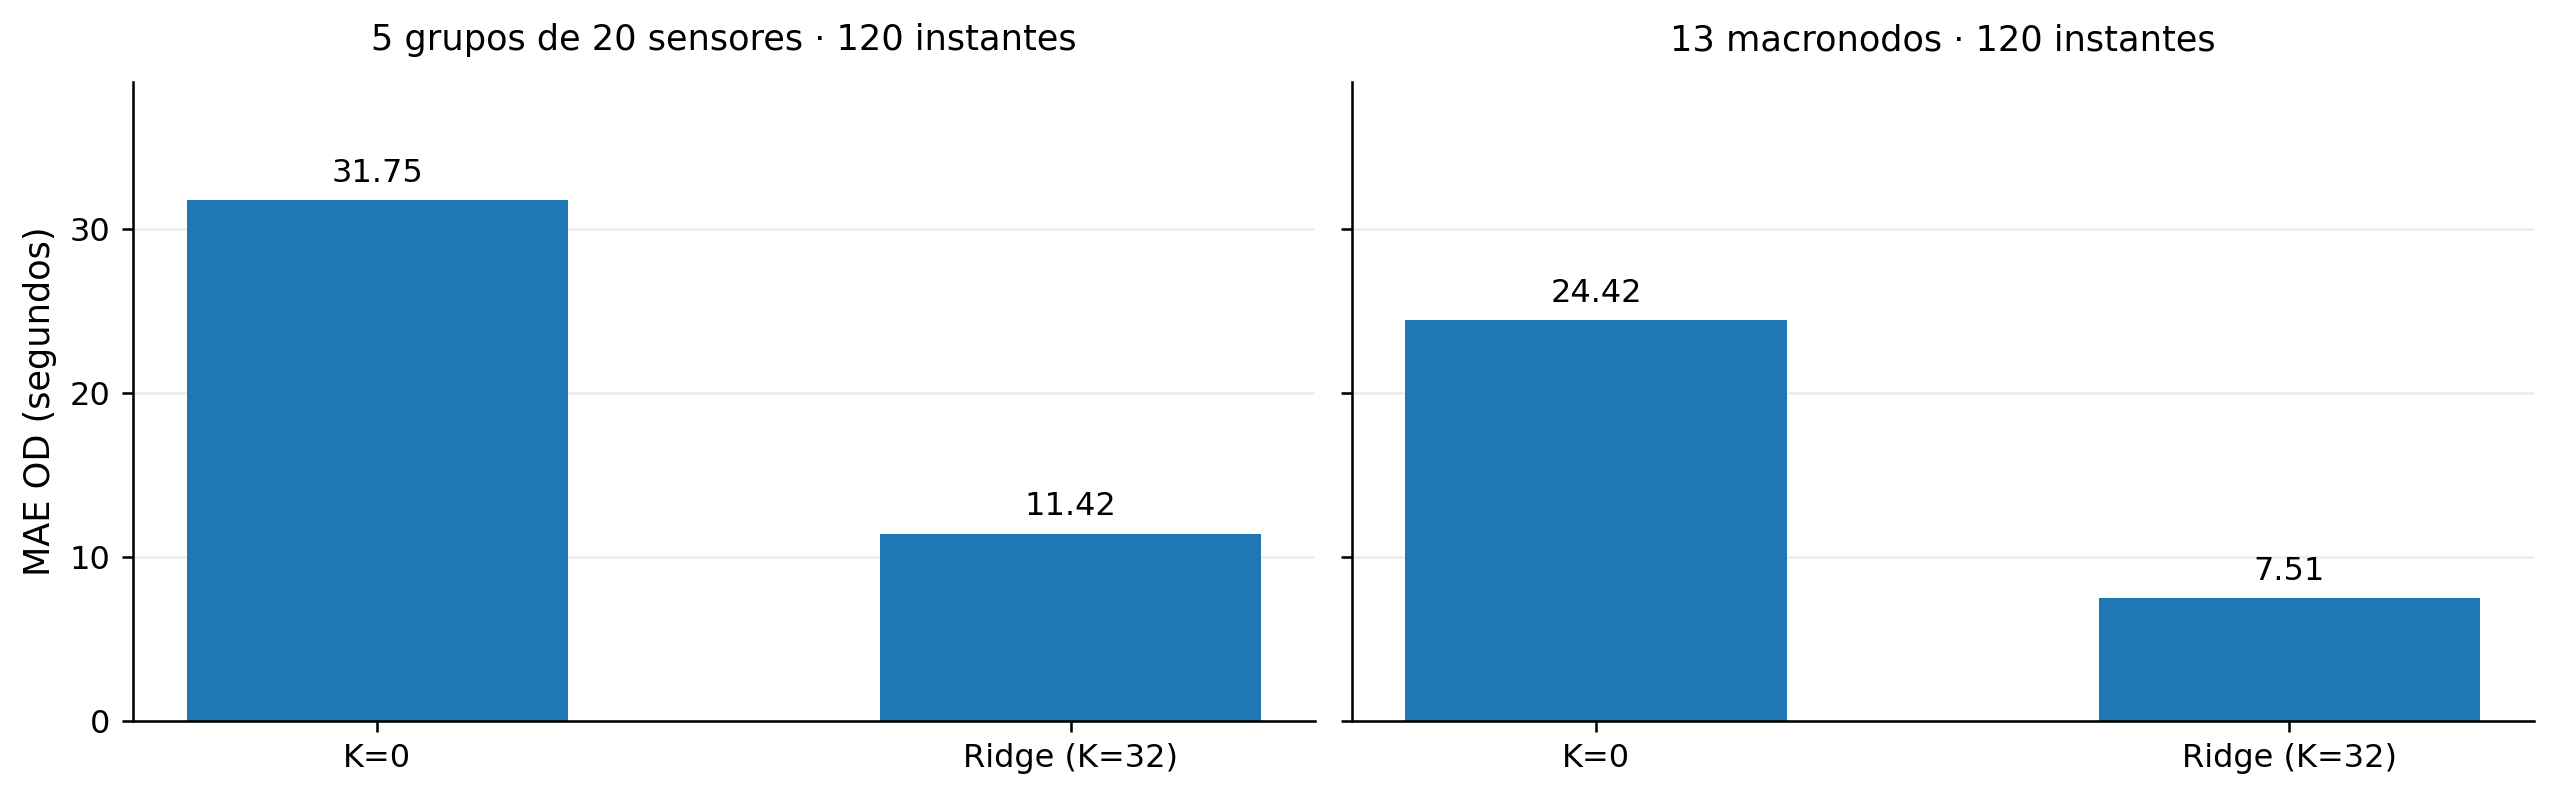
\includegraphics[width=.94\linewidth]{reconstruccion_dos_evaluaciones.png}
\caption{MAE OD de la reconstrucción y su referencia histórica en junio: cinco grupos de sensores (izquierda) y 13 macronodos (derecha). Los paneles corresponden a diferentes conjuntos de pares y muestran el error en una misma escala vertical.}\label{fig:k32}
\end{figure}

K=32 obtuvo un MAE diario inferior a K=0 en los 30 días de junio. Entre las 18\,720 estimaciones OD, la proporción con error absoluto inferior a un minuto aumentó de 89.10\% a 97.69\%, y la de subestimaciones superiores a dos minutos disminuyó de 4.76\% a 0.37\%. Estos umbrales son descriptivos, no requisitos operativos.

\subsection{Evaluación de ensambles}
En los ensambles homogéneos de mayo, el mejor ensamble de tipo \emph{bagging} \parencite{breiman1996} de Ridge presentó MAE OD de 11.4853 segundos frente a 11.5116 de Ridge, una mejora de 0.0263 segundos (0.23\%). Un control de Ridge individual, con regularización ajustada para tener en cuenta que cada modelo del ensamble se entrenó con remuestreos equivalentes al 80\,\% de la muestra original, obtuvo 11.4966. Esto sugiere que parte de la pequeña ventaja podría deberse a la intensidad de la regularización y no solo al promedio de modelos. El mejor ensamble heterogéneo de 75\% Ridge y 25\% KNN, elegido en abril, logró 11.2710 segundos en mayo (2.09\% menor que Ridge). Sin embargo, un intervalo exploratorio de remuestreo en bloques \parencite{kunsch1989} para la diferencia de MAE, de $-0.0395$ a $0.5187$ segundos, incluyó cero. Además, el déficit medio de subestimación aumentó en 0.4390 segundos (intervalo exploratorio de 0.0211 a 0.8535). La mejora de MAE no asegura una mejora uniforme en errores relevantes para ventanas de tiempo. Se conserva Ridge como candidato sencillo para integración, sin atribuir a los ensambles una inferioridad universal.

\subsection{Pronóstico anticipado: comparación de cinco métodos}
La evaluación del pronóstico abarcó 29 jornadas de abril (del 2 al 30, por el protocolo temporal descrito), las 31 de mayo y las 30 de junio de 2017. Cada jornada tiene 96 intervalos y 345 aristas, de modo que cada configuración genera \textbf{2\,980\,800 predicciones arista--instante} en los 90 días. El MAE fue menor para M0 en abril; M1 obtuvo el menor MAE en mayo y junio (Tabla~\ref{tab:pronostico}). En junio, M1 disminuyó el MAE por arista de 2.5981 a 2.4256 segundos (6.64\%); la GNN completa obtuvo 2.5258. Una arquitectura más compleja no garantizó mejor precisión con las configuraciones ensayadas. Abril fue periodo de validación, mientras que mayo y junio deben leerse como diagnósticos del desarrollo, no como pruebas ciegas nuevas.

\begin{table}[htbp]\centering\small
\caption{MAE por arista del pronóstico anticipado, en segundos.}\label{tab:pronostico}
\begin{tabular}{@{}lrrr@{}}\toprule
Modelo & Abril (valid.) & Mayo (diag.) & Junio (diag.) \\ \midrule
M0: mediana histórica & \textbf{1.8894} & 2.5648 & 2.5981 \\
\textbf{M1: lineal residual} & 1.8977 & \textbf{2.4545} & \textbf{2.4256} \\
MLP sin propagación & 1.9371 & 2.5210 & 2.5019 \\
GNN completa & 1.8942 & 2.5081 & 2.5258 \\
GNN sin macronodos & 1.8976 & 2.5039 & 2.5156 \\ \bottomrule
\end{tabular}
\end{table}

En la muestra evaluada, los errores aumentaron en las situaciones definidas como alejadas del patrón histórico. En junio se identificaron 24\,438 pares arista--instante cuyo tiempo de referencia superó al menos 50\% su mediana histórica (2.46\% de ese mes). En ese subconjunto, el MAE de M1 fue 33.486 segundos y el de M0, 35.196: ambos muy superiores a sus medias generales. El criterio del 50\% no es una etiqueta de accidente, obra o cierre constatado. No se dispone de evidencia para afirmar robustez del sistema frente a interrupciones extraordinarias.

\subsection{Evaluación de matrices OD pronosticadas}
Los tiempos pronosticados se utilizaron para generar matrices OD de 13 macronodos y de un único grupo fijo de 20 sensores. Se evaluó una muestra horaria fija de ocho instantes por jornada (08:00, 09:00, \ldots, 15:00), no los 96 intervalos de cinco minutos disponibles; por tanto, las métricas OD solo describen esa muestra. La GNN completa obtuvo el menor MAE OD en abril, con diferencias pequeñas, mientras que M1 lo consiguió en mayo y junio para ambos conjuntos (Tabla~\ref{tab:predod}). El orden de los modelos puede cambiar al acumularse los errores por arista a lo largo de los caminos.

\begin{table}[htbp]\centering\small
\caption{MAE OD del pronóstico anticipado (segundos): ocho instantes por jornada, conjuntos fijos de nodos.}\label{tab:predod}
\begin{tabular}{@{}llrrr@{}}\toprule
Periodo & Conjunto & M0 & M1 & GNN completa \\ \midrule
Abril & 13 macronodos & 26.709 & 26.840 & \textbf{26.518} \\
 & 20 sensores & 35.465 & 35.668 & \textbf{35.228} \\
Mayo & 13 macronodos & 37.315 & \textbf{33.030} & 34.910 \\
 & 20 sensores & 46.816 & \textbf{41.479} & 43.848 \\
Junio & 13 macronodos & 38.150 & \textbf{32.673} & 35.662 \\
 & 20 sensores & 47.692 & \textbf{41.308} & 44.944 \\ \bottomrule
\end{tabular}
\end{table}

Para junio, las 37\,440 predicciones OD de 13 macronodos corresponden a 30 días, ocho instantes diarios y 156 pares dirigidos. Su tiempo de referencia medio fue 634.159 segundos (10.57 minutos). M1 redujo el MAE de 38.150 a 32.673 segundos (14.36\%) y el WAPE de 6.016\% a 5.152\%. La mediana del error porcentual absoluto disminuyó de 2.920\% a 2.055\% y el P95 de 159.644 a 147.667 segundos. M1 redujo la subestimación de 84.084\% a 65.067\% y el sesgo de $-27.130$ a $-16.100$ segundos. \textbf{M1 redujo la suma de errores absolutos OD en 29 de las 30 jornadas} de junio, pero un P95 cercano a dos minutos y medio impide caracterizar sus tiempos como uniformemente precisos.

\subsection{Representación espacial de un instante común}
La Figura~\ref{fig:estados} compara las salidas de los dos componentes a las 08:00 del 6 de junio de 2017, utilizando las estimaciones por arista conservadas en la biblioteca de matrices exportadas y la misma escala cromática. Se representan \emph{velocidades equivalentes calculadas} (distancia aproximada entre nodos dividida entre el tiempo estimado), no velocidades observadas directamente en cada tramo ni tráfico de una operación real. M1 utiliza información disponible antes de la jornada, mientras que K=32 incorpora 32 consultas OD del propio instante, simuladas a partir de los datos de referencia. Por ello, aunque ambas salidas se pueden visualizar simultáneamente, la semejanza de los colores no equivale a una comparación de precisión en igualdad de condiciones. El instante K=32 mostrado proviene de la inferencia ampliada para junio, cuya exactitud no se evaluó exhaustivamente fuera de los 120 instantes de prueba documentados.

\begin{figure}[htbp]\centering
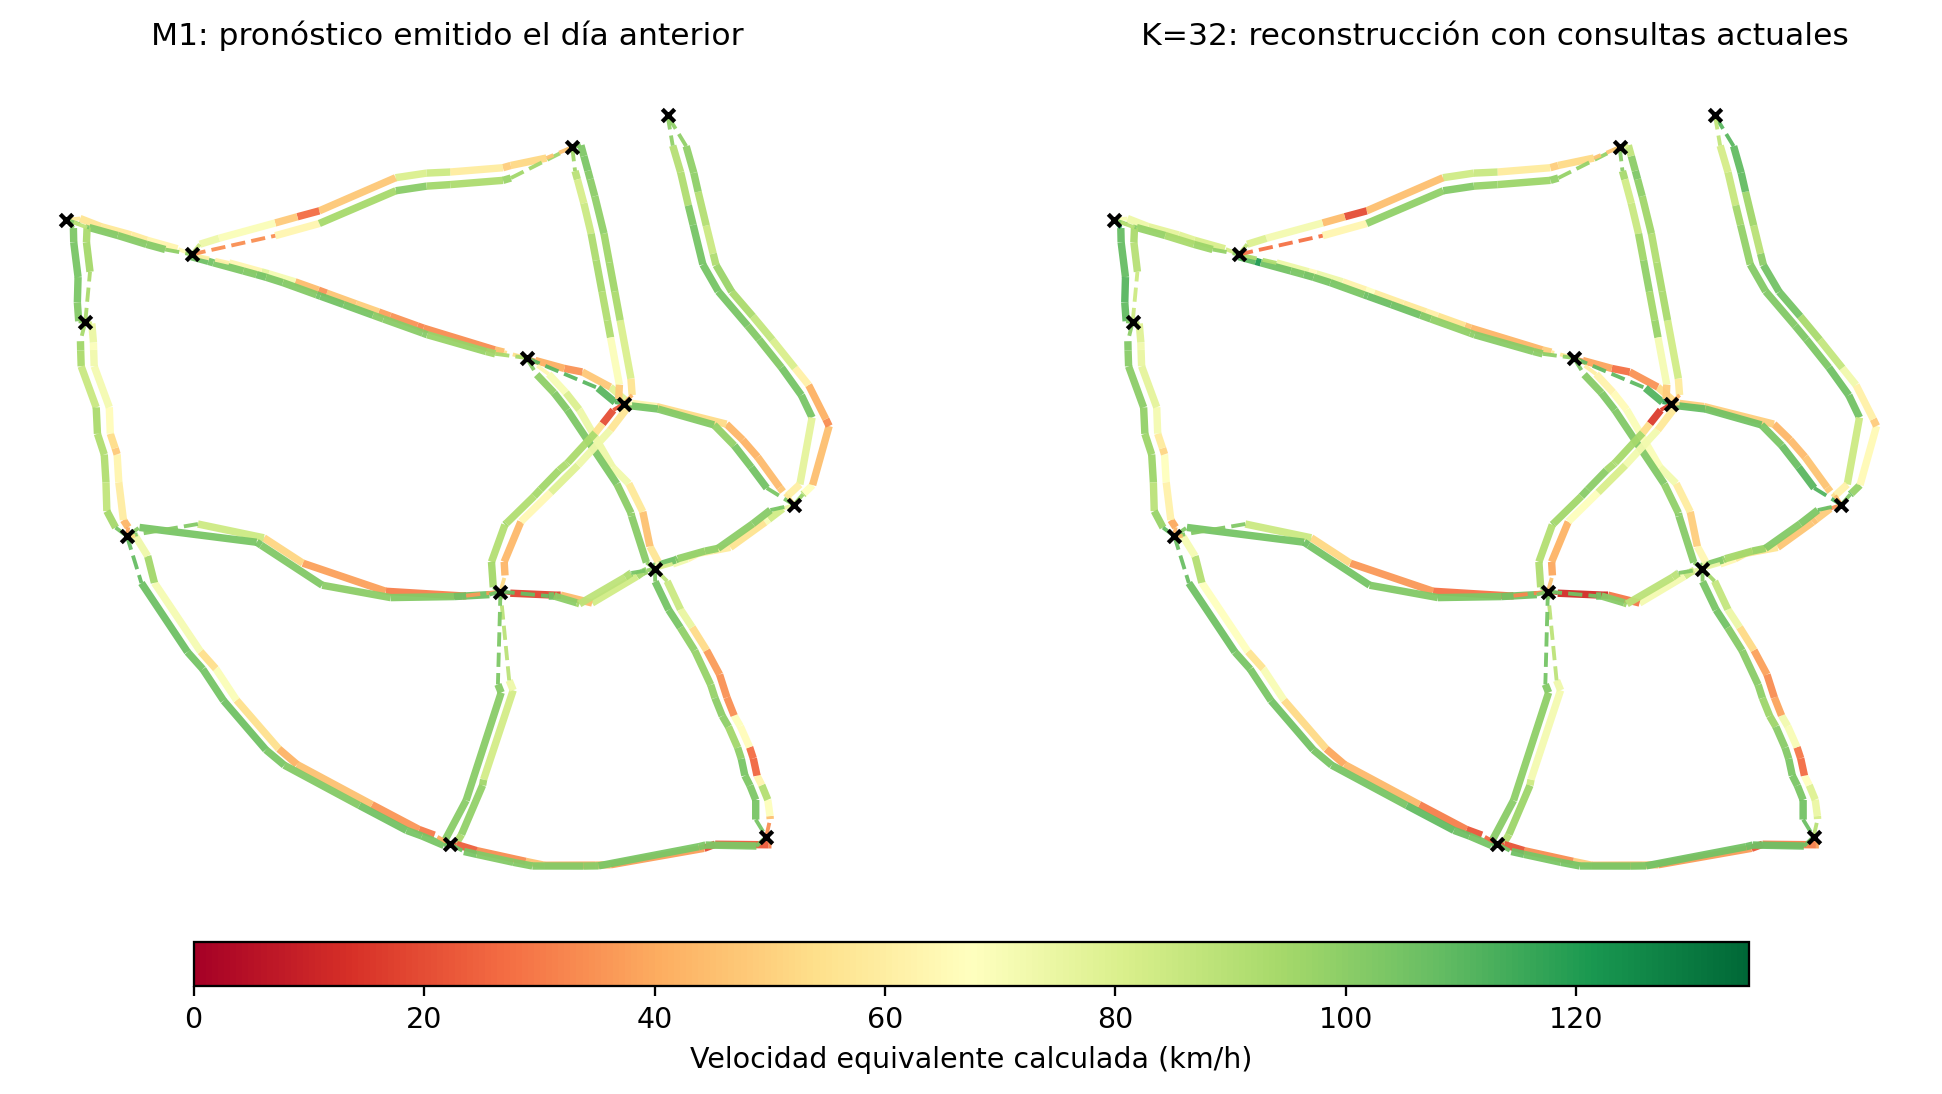
\includegraphics[width=\linewidth]{estados_M1_K32_mismo_instante.png}
\caption{Representación del estado estimado de la red el 6 de junio de 2017, 08:00: pronóstico anticipado M1 (izquierda) y reconstrucción contemporánea K=32 (derecha). Ambos paneles emplean la misma topología y escala de velocidad equivalente calculada; se distinguen por el momento en que está disponible su información de entrada.}\label{fig:estados}
\end{figure}


\subsection{Condiciones de circulación y límites del desempeño}
Para examinar cómo varía el error según las condiciones de tráfico, se construyó un indicador de lentitud relativa de la red. En cada instante se dividió la suma de los tiempos de referencia de las aristas de corredor entre la suma de sus tiempos históricos correspondientes. Un cociente mayor indica circulación más lenta respecto del patrón habitual. A partir de sus percentiles 10 y 90 se distinguieron tres grupos de instantes: 10\% de menor lentitud, 80\% intermedio y 10\% de mayor lentitud. Los cortes se calcularon por separado para cada componente y la clasificación fue retrospectiva; no identifica incidentes ni constituye información disponible al emitir un pronóstico.

La Figura~\ref{fig:reg} presenta el WAPE OD por grupo. En M1, el mayor error correspondió a los instantes de mayor lentitud (11.47\%), mientras que en los de menor lentitud fue ligeramente superior al de M0 (7.38\% frente a 7.17\%). En K=32, el WAPE disminuyó respecto de K=0 en los tres grupos y pasó de 11.21\% a 2.76\% en el de mayor lentitud. No obstante, ese 10\% de instantes concentró 26.94\% del error absoluto de K=32.

\begin{figure}[htbp]\centering
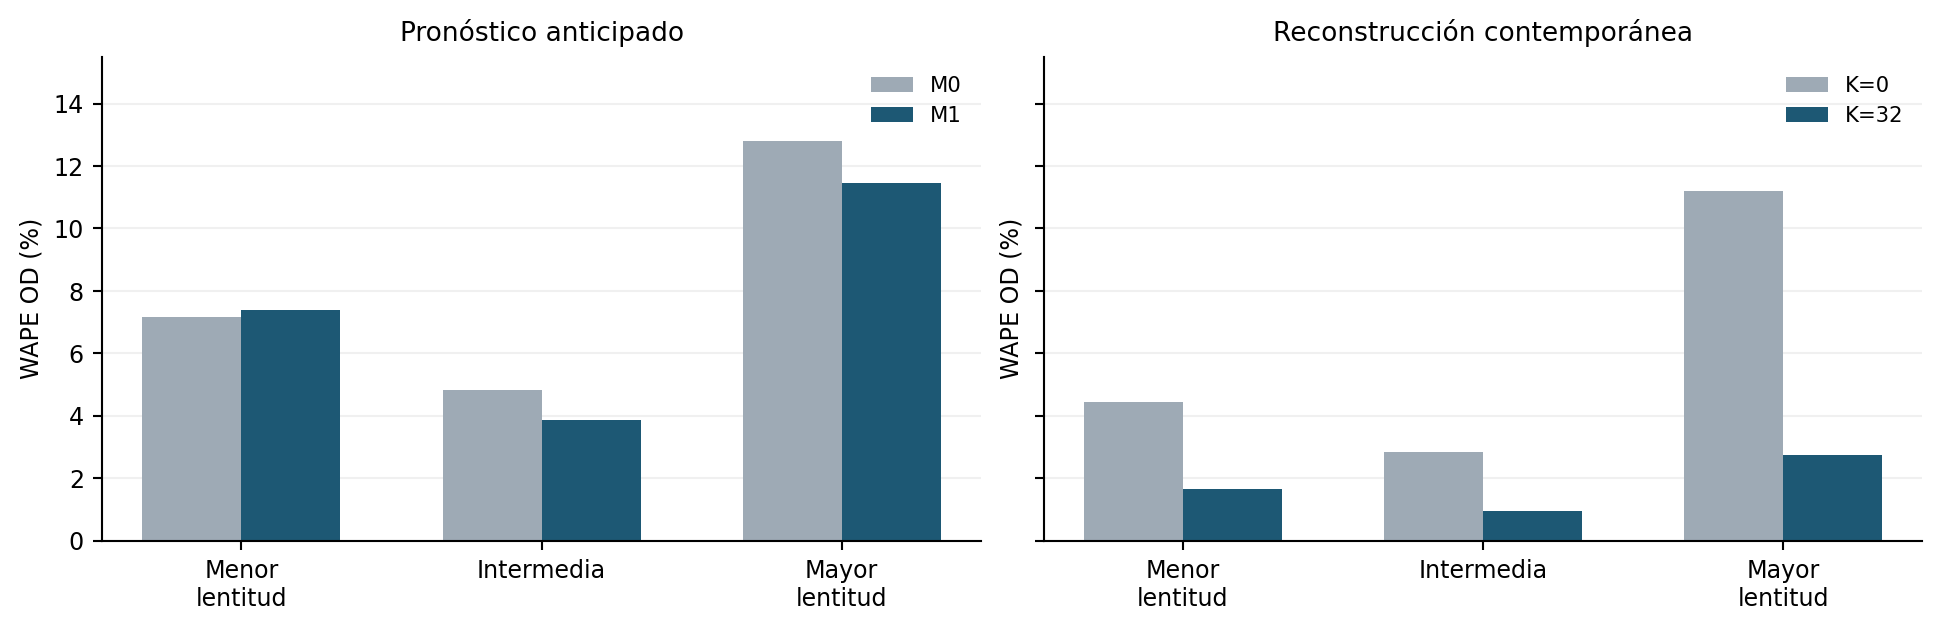
\includegraphics[width=.96\linewidth]{regimenes_lentitud.png}
\caption{WAPE OD de la reconstrucción contemporánea y del pronóstico según tres niveles de lentitud relativa (10\% menor, 80\% intermedio, 10\% mayor). Los regímenes se definieron retrospectivamente y por separado para cada componente.}\label{fig:reg}
\end{figure}

La concentración de errores en situaciones de mayor lentitud aconseja evaluaciones específicas antes de emplear estas matrices en decisiones con ventanas de servicio estrechas. Para ello se requerirían episodios independientes y criterios operativos establecidos previamente.


\subsection{Discusión y alcance de los resultados}
La reducción del error de una matriz OD no se traduce automáticamente en mejores rutas. Una diferencia de 30 segundos puede ser irrelevante cuando existe holgura suficiente o decisiva si la ventana de servicio está próxima a cerrarse. Además, cambiar los tiempos estimados puede modificar la secuencia elegida por un optimizador. Por ello, la utilidad logística deberá medirse comparando rutas construidas con distintas matrices y evaluándolas después con tiempos de referencia, no solo mediante MAE o WAPE.

La subestimación merece especial atención. En junio, M1 presentó un sesgo OD de $-16.100$ segundos y subestimó aproximadamente el 65\% de los tiempos entre macronodos; el P95 del error absoluto fue de 147.667 segundos. Una ruta con poca holgura podría verse afectada, aunque estos indicadores no permiten calcular incumplimientos sin conocer servicios, secuencias y ventanas. En la evaluación complementaria de K=32, el sesgo medio fue cercano a cero, pero el 36.095\% de sus estimaciones también quedó por debajo de la referencia.

Las comparaciones deben interpretarse dentro de sus respectivas muestras: la evaluación principal de K=32 utilizó pares entre sensores distintos de los consultados, su evaluación complementaria incluyó pares guía y M1 se examinó sobre ocho horarios OD por jornada. Los dos procedimientos reciben información de distinta antigüedad y no se compararon directamente. Además, los pares de una misma red y jornada comparten condiciones y segmentos; las numerosas observaciones OD no constituyen réplicas independientes. Una evaluación confirmatoria deberá reservar nuevos periodos o episodios y considerar esa dependencia estadística.

\section{Artefactos generados y condiciones de implementación}

\subsection{Artefactos producidos y verificación}
Se prepararon catálogos de nodos y aristas, funciones Python para calcular caminos mínimos dirigidos, matrices OD de ejemplo y una biblioteca de tiempos estimados por arista para junio de 2017, acompañada de metadatos. El paquete \texttt{entrega\_matrices\_OD\_optimizador} contiene 11\,520 registros \emph{modelo--instante}: 2\,880 de M1 para los 96 intervalos de 08:00 a 15:55 durante 30 jornadas y 8\,640 de K=32 para los 288 intervalos diarios. A partir de estos registros pueden calcularse matrices para los nodos y horarios solicitados, con tiempos OD en minutos e identificación temporal.

La ampliación de K=32 a 8\,640 instantes supuso 2\,980\,800 estimaciones arista--instante, pero no constituye una evaluación adicional de precisión. Se comprobó la reproducción de las predicciones en los 120 instantes originales y se registraron 230 reemplazos de tiempos no positivos (0.0077\%) por su referencia histórica. El paquete conserva estimaciones experimentales de junio de 2017, no datos actuales ni consultas OD obtenidas de un servicio externo.


\subsection{Condiciones para la integración con el optimizador}
El optimizador de recuperación de rutas de Berth y Trigos no se implementó ni ejecutó en este trabajo. Para una integración será necesario relacionar los nodos experimentales con depósitos y clientes, definir sus identificadores y orden, acordar unidades y redondeos, y resolver los casos de pares no alcanzables y movimientos viales no permitidos. También deben precisarse el momento de salida, el formato de intercambio, el manejo de errores y, para K=32, la disponibilidad y latencia de consultas externas. Que un optimizador pueda leer una matriz no garantiza que interprete correctamente sus supuestos temporales ni sus restricciones viales.

Una prueba inicial podría utilizar una instancia pequeña y reproducible de recuperación, con las mismas demandas, capacidades, ventanas de servicio y estado de ejecución, modificando únicamente los tiempos de viaje: referencia histórica frente a estimaciones. Se compararían factibilidad, retrasos, costo de recuperación y latencia total. Solo después de esa evaluación sería pertinente examinar posibles beneficios operativos.


\subsection{Limitaciones, riesgos y criterios pendientes}
Las limitaciones afectan a la referencia, la validación y la operación. Los tiempos OD de referencia proceden de velocidades de sensores y caminos calculados, no de viajes observados independientemente; además, las conexiones funcionales entre corredores no se contrastaron de manera exhaustiva. En la reconstrucción, junio se reservó para la evaluación principal después de seleccionar el modelo, pero la evaluación complementaria reutilizó esos instantes e incluyó pares consultados. En el pronóstico, abril se utilizó para validación y mayo--junio para diagnósticos examinados durante el desarrollo. Por su parte, las 32 consultas de K=32 son exactas y simuladas: aún se desconocen la precisión, disponibilidad, costo y latencia de observaciones externas.

Un piloto debería establecer previamente criterios de aceptación para errores OD, subestimaciones, cobertura de datos y tiempos de respuesta, además de verificar el efecto sobre la factibilidad de las rutas. Se necesitarían mecanismos de respaldo ante datos faltantes o estimaciones inválidas y supervisión durante las pruebas.

La exploración de los registros LCS quedó pendiente de integración debido al tiempo disponible para el proyecto. Como trabajo futuro, corresponde reconstruir qué solicitudes y estados administrativos habrían sido conocidos antes de cada pronóstico, mejorar su correspondencia temporal con la red y evaluar si las variables resultantes aportan información predictiva adicional a los registros de tráfico.


\section{Conclusiones y trabajo futuro}
Se construyó una red experimental dirigida y se desarrollaron dos procedimientos para generar matrices de tiempos de viaje en distintos momentos de decisión. En la reconstrucción contemporánea, Ridge con 32 consultas OD simuladas redujo 64.04\% el MAE frente a la referencia histórica en la evaluación principal de junio, realizada sobre cinco grupos de sensores cuyos pares no coincidían con los consultados. La evaluación complementaria entre macronodos mostró una reducción de 69.27\%, aunque incluyó los pares guía. Para el pronóstico de la jornada siguiente, M1 redujo 14.36\% el MAE OD respecto de la mediana histórica en junio, sobre 13 macronodos. Estas mejoras corresponden a protocolos distintos y no comparan directamente ambos procedimientos.

El trabajo aporta métodos de estimación documentados, una representación temporal de la red y matrices exportables para pruebas posteriores. Los resultados también muestran desafíos: la precisión varía con las condiciones de circulación, persisten subestimaciones y las consultas contemporáneas solo se estudiaron en un entorno simulado. Las arquitecturas más complejas y los ensambles no demostraron una ventaja suficientemente consistente para desplazar a los modelos seleccionados.

La continuación prioritaria consiste en integrar las matrices a una instancia de recuperación de rutas con ventanas de tiempo y medir sus efectos sobre factibilidad, retrasos y costo frente a una referencia histórica. También corresponde contrastar consultas externas y examinar episodios de circulación atípica y la información contextual del LCS. Así podrá determinarse si las mejoras de estimación se traducen en beneficios para la toma de decisiones, cuestión todavía abierta.

\section*{Declaración de uso de inteligencia artificial}
Se utilizaron ChatGPT (OpenAI) y Claude (Anthropic) como apoyo en la búsqueda de literatura, el desarrollo y depuración de código, los análisis y pruebas computacionales de los Avances, la elaboración de tablas y figuras, y la revisión y redacción de la documentación y del archivo LaTeX. En el artículo final no se realizaron nuevos experimentos: se consolidaron resultados ya documentados. Las decisiones metodológicas, la interpretación de los hallazgos, la revisión de las fuentes y las conclusiones son responsabilidad de los autores.

{\setstretch{1.0}\setlength{\bibitemsep}{0pt}\printbibliography[title={Referencias}]}
\clearpage
\appendix

\section{Materiales complementarios y trazabilidad de resultados}
\label{app:traza}

Los materiales técnicos que respaldan este artículo se organizan en el repositorio del Equipo 42, disponible en \url{https://github.com/Luis-MX/route-intelligence}. Las entregas académicas se encuentran en el directorio \href{https://github.com/Luis-MX/route-intelligence/tree/main/docs/entregas}{\texttt{docs/entregas}}, con una subcarpeta para cada avance. Estas reúnen informes, cuadernos de Jupyter, archivos fuente y otros materiales desarrollados durante las distintas etapas del proyecto.

La Tabla~\ref{tab:traza} relaciona los principales resultados del artículo con los materiales que documentan su obtención y evaluación. Los avances 3 a 6 contienen los procedimientos experimentales desarrollados durante el curso, mientras que el Avance 7 reúne el artículo académico, los materiales de difusión y la libreta de análisis complementario de M1 y $K=32$, que también documenta las verificaciones asociadas con la generación de matrices OD.

\begin{table}[H]
\centering
\footnotesize
\renewcommand{\arraystretch}{1.10}
\caption{Mapa de evidencias del artículo y materiales técnicos de respaldo.}
\label{tab:traza}

\begin{tabular}{@{}
>{\raggedright\arraybackslash}p{.25\linewidth}
>{\raggedright\arraybackslash}p{.27\linewidth}
>{\raggedright\arraybackslash}p{.40\linewidth}
@{}}
\toprule
Evidencia del artículo &
Material de respaldo &
Contenido documentado \\
\midrule

Red, velocidades y tiempos de arista (Secc.~2) &
Informe y cuadernos de preparación
(\href{https://github.com/Luis-MX/route-intelligence/tree/main/docs/entregas/avance-3-baseline}{Avance 3}) &
Depuración de velocidades, continuidad temporal, construcción de corredores y macronodos, y cálculo de tiempos por arista. \\

Referencia histórica y reconstrucción inicial (Secc.~3) &
Informe y cuadernos técnicos
(\href{https://github.com/Luis-MX/route-intelligence/tree/main/docs/entregas/avance-3-baseline}{Avance 3}) &
Selección de granularidad temporal, medianas históricas y evaluación preliminar de tiempos OD. \\

Selección de consultas y Ridge; reducción de 64.04\,\% (Seccs.~3--4) &
Cuaderno de reconstrucción
(\href{https://github.com/Luis-MX/route-intelligence/tree/main/docs/entregas/avance-4-modelos-alternativos}{Avance 4}) &
Selección progresiva de consultas, comparación de valores de $K$, modelos alternativos y evaluación principal de junio. \\

Ensambles y alternativas (Secc.~4) &
Cuadernos de ensambles
(\href{https://github.com/Luis-MX/route-intelligence/tree/main/docs/entregas/avance-5-ensambles-y-contexto}{Avance 5}) &
Ensambles homogéneos y heterogéneos, regularización, combinación Ridge--KNN y remuestreo exploratorio. \\

Información administrativa LCS (Secc.~2) &
Cuaderno de correspondencias espaciales
(\href{https://github.com/Luis-MX/route-intelligence/tree/main/docs/entregas/avance-5-ensambles-y-contexto}{Avance 5}) &
Solicitudes administrativas, asociaciones con aristas de corredor y exploración de su posible utilidad predictiva. \\

Pronóstico anticipado M1 (Seccs.~3--4) &
Cuaderno y documentación técnica
(\href{https://github.com/Luis-MX/route-intelligence/tree/main/docs/entregas/avance-6-prediccion-jornada-siguiente}{Avance 6}) &
Protocolo de emisión, características predictivas, comparación de modelos y evaluación de abril--junio. \\

Evaluaciones complementarias y condiciones de circulación (Secc.~4) &
\href{https://github.com/Luis-MX/route-intelligence/tree/main/docs/entregas/avance-7-proyecto-de-difusion}{Avance 7}: libreta de análisis complementario &
Evaluación de $K=32$ entre 13 macronodos, análisis de errores, regímenes de lentitud relativa y comparación espacial con M1. \\

Matrices OD exportables (Secc.~5) &
\href{https://github.com/Luis-MX/route-intelligence/blob/main/docs/entregas/avance-7-proyecto-de-difusion/Analisis_complementario_M1_K32_y_matrices_OD_Equipo42.ipynb}{Libreta de análisis complementario}
(\href{https://github.com/Luis-MX/route-intelligence/tree/main/docs/entregas/avance-7-proyecto-de-difusion}{Avance 7}) &
Ampliación de estimaciones de junio, generación de matrices OD, catálogos, metadatos y verificaciones de consistencia. \\

\bottomrule
\end{tabular}
\end{table}


\section{Reproducibilidad y condiciones de interpretación}\label{app:cond}
Para reproducir las métricas deben conservarse los periodos de ajuste, los grupos de sensores y macronodos, los pares dirigidos y los instantes evaluados. Las dos evaluaciones de K=32 usan el mismo modelo y 120 instantes, pero diferentes pares OD; la complementaria incluye las consultas guía. M1 sigue otro protocolo temporal. Las 32 consultas se calcularon con los mismos tiempos de arista utilizados como referencia y no equivalen a mediciones OD externas.

La ampliación de K=32 a otros instantes de junio produce matrices, no una evaluación adicional de precisión. Las métricas proceden de los cuadernos relacionados en la Tabla~\ref{tab:traza}; para reproducirlas deben comprobarse las versiones y las rutas de los archivos disponibles en el repositorio.
\end{document}
